\subsection{The shortcut approach}

After the problem with layers crossed our path in the first attempt, we took a step back and tried to reevaluate our approach. The second attempt is based on looking at elements of alternatives (the concept placeholders themselves) and asking "which concepts could be inserted here?". Consider again the \parserrule{content} rule and its children rules:

\begin{antlr}
	\parserrule{content}    :   \lexerrule{TEXT}
           |   \parserrule{element}
           |   \parserrule{comment}
           |   \lexerrule{CDATA}
           ;
	
	\parserrule{element}    :   \literal{<} \lexerrule{Name} \parserrule{attribute}* \literal{>} \parserrule{content}* \literal{</} \lexerrule{Name} \literal{>}
           |   \literal{<} \lexerrule{Name} \parserrule{attribute}* \literal{/>}
           ;	
	
	\parserrule{comment}    :   \literal{<!--} \lexerrule{TEXT} \literal{-->} ;
\end{antlr} 

We can see that the content rule can ultimately expand into following concepts: 

\begin{itemize}
	\setlength\itemsep{0pt}
	\item Content{\_}1
	\item Element{\_}1
	\item Element{\_}2
	\item Comment
	\item Content{\_}4
\end{itemize}

These are concepts that can directly appear for example inside the XML element which we would like to see in the auto-completion menu. They cannot break into more rules and for the sake of text we will call them \textbf{end concepts}, or when talking about the grammar rule tree \textbf{end rules}.

\subsubsection{The algorithm}
To find these end concepts, we can recursively scan through the parser tree that we have built before. For each parser rule, we will try to find paths leading to some end rule through its alternatives:

\begin{itemize}
	\item Whenever we find an alternative that contains only one element and this element is a reference to another parser rule, we have found an intermediary level that can be later somehow transparently hidden from the user of the language. We will continue recursively processing alternatives of this “level” rule. 
	
	\item Otherwise, we have found an end rule (recursion stops here). 
\end{itemize}
	
We have expressed this algorithm using a pseudo-code:

\label{chap:shortcut_algorithm}
\begin{antlr}
FindPathsToEndNodes(\textit{R}):
   1)  Define \textit{L} as an empty list of list of nodes
   2)  Return FindPathsToEndNodes(\textit{R}, \textit{L})

FindPathsToEndNodes(\textit{R}, \textit{L}):
   3)  Define \textit{Q} as list of list of nodes
   4)  For each alternative \textit{A} of rule \textit{R}:
   5)      Copy \textit{L} to \textit{L1}
   6)      If \textit{A} is a parser rule with only one element \textit{E}: 
   7)          Let \textit{I} be interface/concept representing rule \textit{E}
   8)          \textit{L1}.Add(\textit{I})
   9)          \textit{P} = FindPathsToEndNodes(\textit{E}, \textit{L1})
  10)          \textit{Q} = Merge(\textit{Q}, \textit{P})
  11)      Else
  12)          \textit{L1}.Add(\textit{R})
  13)          Let \textit{P} be concept representing \textit{A}
  14)          \textit{L1}.Add(\textit{P})
  15)          \textit{Q}.Add(\textit{L1})
  16)  Return \textit{Q}
\end{antlr}

By appending the rule that is leading to current element (line 12) and then appending the alternative’s element itself (line 14), we will get a path that contains the full path and the target end node as the last element.
\\

We can do this for all parser rules and for each rule we will get a list of paths that lead from that particular rule to an end node. We will call these paths shortcuts. Now that we have these, we will talk about several ways how to use them to make our language better.

\subsubsection{Smart auto-completion}
The first attempt on how to use shortcuts was built on top of the previous approach. There were no structural changes when it came to interface or concept definition. We imported everything just the same and then added some more functionality.

We were trying to solve the most obvious problem in front of us --- the auto-completion, where we were offered options that were not end concepts. Luckily for us, MPS gives us the ability to create own auto-complete menus and use those instead of the built-in one. This means, that we are going to be able to construct our own menu containing only end nodes. Unfortunately, it requires us to implement some non-trivial mechanisms. 

\paragraph{Defining the auto-complete}

The auto-complete menu is bound to a cell of the projectional editor containing a reference to one of the children of a concept. Let's say we are again talking about the concept that represents the element rule's first alternative. As described above earlier in the process, we created:

\begin{itemize}
	\setlength\itemsep{0pt}
	
	\item An interface \interface{IContent} representing four different alternatives that the content rule can break into
	
	\item A child of the \concept{Element{\_}1} concept, that references the \interface{IContent} rule
\end{itemize}
 
Somewhere in the editor aspect of the \concept{Element{\_}1} concept, there will be a cell referencing the concept interface \interface{IContent}. We would like to create an auto-complete for this cell that would contain following options (end concepts):

\begin{itemize}
	\setlength\itemsep{0pt}
	\item Content{\_}1
	\item Element{\_}1
	\item Element{\_}2
	\item Comment
	\item Content{\_}4
\end{itemize}

Because we are inside MPS everything is a concept node. In order to create an auto-complete menu, we need to create some BaseLang code, more precisely an instance of some concept from one of many MPS's core languages that are used to build MPS itself (MPS is self-hosting). There is a concept called [TODO auto-complete menu concept name] that represents the auto-complete menu. 
\\

For this concept we will define a number of auto-complete options, one for each end concept we want to offer in the menu. Every option has a textual description, matching text so that we can filter through them and most importantly a creator method. If user selects that particular option, this method will be called with some contextual information in parameters and it is expected to return an instance of some concept that implements the \interface{IContent} interface.
\\

The complicated part of the process comes now as we would like to dynamically generate instructions of the creator method. We need to create statements that will instantiate the end concept and return it. There is one small problem though. Let's say the user selected the second option and decided to insert another \concept{Element{\_}1} inside the content. The problem is that \concept{Element{\_}1} doesn't implement the \interface{IContent} interface. It only implements the Element interface as per the algorithm of the straightforward approach (\ref{chap:straight_algorithm}). The shortcut that leads to this end concept leads through the \concept{Content{\_}2} concept, that has an Element child. This means, that we have to follow the whole shortcut (starting at the end, going backwards) and chain individual nodes. For this particular case it would mean to:

\begin{itemize}
	\item Create an \concept{Element{\_}1} concept and store it in a variable
	
	\item Create a \concept{Content{\_}2} concept and store it in a variable
	
	\item Assign the \concept{Element{\_}1} node to the right child of the \concept{Content{\_}2} node
	
	\item Return \concept{Content{\_}2} node
\end{itemize}

As we said earlier in section \ref{chap:generating_code_inside_mps}, generating BaseLang code is a bit more complicated because we need to either use quotation or create a large number of AST nodes. Using quotation in this case was sometimes impossible as everything is very dynamic. The finished option concept is shown in figure \ref{fig:autocomplete_action}.

\begin{figure}[h]
	\centering
	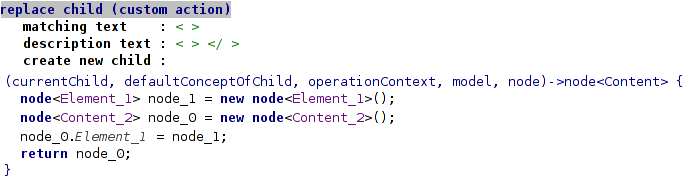
\includegraphics[width=\textwidth]{../img/autocomplete_action.png}
	\caption{Auto-complete action code (Element{\_}1 concept)}
	\label{fig:autocomplete_action}
\end{figure}

For description text, we used concept's alias. We talk about creating aliases in chapter [TODO: alias chapter reference]. For matching text we used the shortest unique prefix of alias among all other options' aliases in given auto-complete menu. The algorithm for searching shortest unique prefixes in a set of strings is not important from our thesis' point of view, so we decided to not go into further detail.

\paragraph{The layer problem again}

After we implemented the auto-complete menu, coding in the imported language started to be very reasonable and comfortable since we eradicated intermediate layers. Or did we? When producing code, the language really does what one would expect, however when user starts deleting things, the layer problem occurs once more. 
\\

What happens here is that when we select the auto-complete option, several layers of concept might get created and inserted into the cell. Imagine we just inserted the \concept{Element{\_}1} node. According to the creator method, this new node is wrapped inside of the \concept{Content{\_}2} node. Now let's say user changed his mind and wants to replace this XML element with a comment. He would press backspace, the XML element would disappear as expected. Then user would invoke the auto-complete menu again and expect again to have all five options at hand. What happened instead is that the \concept{Element{\_}1} node got deleted, but the wrapping \concept{Content{\_}2} one remained. The \concept{Content{\_}2} concept has only one child of type Element and that is why user only sees \concept{Element{\_}1} and \concept{Element{\_}2} as options in the auto-complete.

\paragraph {The deletion context}

Solution to this resurrected layer problem lies in controlling the deletion event. Once again, MPS' authors have equipped us with tools for doing this. We are able to specify our own handler for the deletion event for any cell of the projectional editor. But what will it look like?
\\

When deleting a node, we would like to remove the shortcut, the whole path, and effectively reversing the effect of the creator method. We decided that it will be the easiest to store the length of the path that is leading to certain node with the node. So when we are creating the node path in the creator method, we tell each node how deep or far on the path it is. In order to do this, we created a \concept{BaseConcept}, a parent abstract concept from which we will inherit all other concepts. This abstract concept will define a special integer property that will hold our information and effectively making all other concepts inherit it too. We called this property \textit{{\_}{\_}DeleteContext} and enhanced the creator method as shown in figure \ref{fig:autocomplete_action_delete_context}.

\begin{figure}[h]
	\centering
	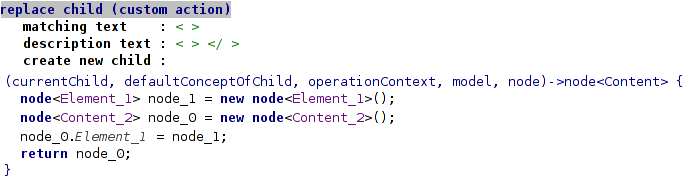
\includegraphics[width=\textwidth]{../img/autocomplete_action_delete_context.png}
	\caption{Auto-complete action extended with deletion context}
	\label{fig:autocomplete_action_delete_context}
\end{figure}

The last thing remaining is creating the backspace action. Apart from some problems with referencing the \textit{{\_}{\_}DeleteContext} property, which must be reached through the abstract \concept{BaseConcept} type, it is quite straightforward to generate a BaseLang code like shown below (figure \ref{fig:backspace_action}).

\begin{figure}[h]
	\centering
	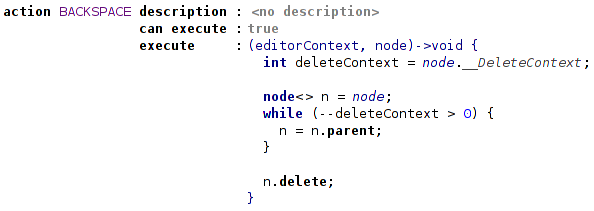
\includegraphics[width=\textwidth]{../img/backspace_action.png}
	\caption{Backspace action implementation}
	\label{fig:backspace_action}
\end{figure}

We must not forget to pin this handler to every cell that we pin the auto-complete to. After we had done this, the layer problem has finally been eradicated. The language became a bit more usable once more.

\subsubsection{Smart interfaces}

After we have implemented the smart autocomplete, we realized that there might be another way to accomplish almost the same result. It would mean changing the first step concerning concept interfaces creation. 
\\

The main idea behind this is the realization that if for each concept interface there exists a finite set of end concepts, we could just create a special interface and let all these and only these end concepts implement it. It is important that other non-end concepts that are in the shortcut will not implement it, because that would put us right back where we started with the straightforward approach \ref{chap:straightforward_approach} and the layer problem \ref{chap:layer_problem}. To give an example regarding our content rule, we would create an \interface{IContent} interface concept and only following concepts would implement it:

\begin{itemize}
	\setlength\itemsep{0pt}
	\item Content{\_}1
	\item Element{\_}1
	\item Element{\_}2
	\item Comment
	\item Content{\_}4
\end{itemize}

Concepts would of course implement as many interfaces as many shortcuts lead to them. The difference is that the intermediary layers will not, preventing the layering.
\\

We still need to find end concepts for each rule, so we will keep the same algorithm for finding shortcuts as before. We, however, do not need to implement our own auto-completion (and subsequently with it no deletion handlers), because the built in default auto-completion will start to behave exactly the same way our smart auto-completion did.

\paragraph{Cardinality restriction}

So far it looks like the last approach is superior to the auto-completion one. It avoids complicated code generation and even resulting MPS languages are more simple, perhaps better performant as they are not bloated with auto-completion code. There is one small drawback though, that makes this solution suboptimal.
\\

To remind the reader --- the cardinality of an element is telling us, how many of each specific child rules can occur inside an alternative. Inside the grammar this was expressed using quantification operators (\textbf{*},\textbf{+} and \textbf{?}). The problem that appears here can be shown using these example rules:

\begin{antlr}
\parserrule{content}      :   \parserrule{element}+
             |   \parserrule{comment}*
             |   \lexerrule{CDATA}?
             ;
\end{antlr}	

Notice, how we changed the cardinality of elements inside the \parserrule{content} rule. This small change will prevent us from creating a shortcut leading through this rule. We are trying to say that shortcuts that can be used for the smart interfaces approach can only lead through rules, that have cardinality [1..1] (so through an alternative with a single child element, that is a reference to a parser rule AND has this cardinality). Speaking in terms of the shortcut algorithm \ref{chap:shortcut_algorithm}, we would alter line number 6 and add this restriction to the condition.
\\

This restriction is caused by the fact that we would be unable to control children cardinality. Imagine that some alternative of some other rule contains reference to this altered \parserrule{content} rule (regardless of its quantitative operator). That means that we need to create a child holding the \interface{IContent} and setting this cardinality. But each alternative of the altered content rule requires different number of children to be inserted. Since there are no intermediary levels of nodes that could influence this, the end concept node that would be inserted in that child would inherit the cardinality of the child regardless of what the shortcut path looks like.
\\

A small example might demonstrate this better. We have an \interface{IContent} [1..1] child. If we disregarded the cardinality restriction, we could ultimately put there \concept{Element{\_}1} end concept node. But the content rule says, there can be [1..n] elements. We are still bound to insert only one though. 

\subsection{Our solution}

In the end, we have decided to go with the solution of smart interfaces. As we have stated above, it has several advantages concerning complexity compared to the smart auto-completion and only one disadvantage regarding the cardinality restriction. Even though it is slightly suboptimal, we have analyzed several ANTLR grammars (such as JavaScript \footnote{https://github.com/antlr/grammars-v4/blob/master/ecmascript/ECMAScript.g4}) and we haven't found a single intermediate rule that would be breaking this condition. It is quite understandable if you think about how grammars are written. Usually, you create the basic structure (i.e. different kinds of statements) in the simplest way possible and put the quantitative operator rather to an alternative that is referencing the structure. It would make thing very complicated and messy to have it randomly around. And more importantly, that is just not the way languages look like. 
\\

Based on these observations and some grammar analysis, we concluded that advantages prevail and went with the last mentioned approach.

\subsection{Structure aspect and advanced ANTLR features}

The ANTLR grammar notation offers more features than just rule definition. We haven't mentioned these earlier because we were focusing on the structure of the language. We will mention some features and explain why we have ignored them and why they doesn't matter to us. We will not spend a lot of time on describing details of these as they are well documented in the official ANTLR reference \footnote{https://github.com/antlr/antlr4/blob/master/doc/index.md}.

\subsubsection{Modes}

For example, just like any other parser/lexer, ANTLR gives us the possibility to switch the parsing context. We are able to create various user specified modes and then enter these modes when certain rules/tokens are encountered. For each mode we can define different set of rules/tokens that can only be applied when the parser is in that particular mode. The syntax is following:

\begin{antlr}
\textcolor{gray}{// Enter mode when tag opened}
\lexerrule{OPEN}        :   \literal{<}       -> pushMode(INSIDE) ;

mode INSIDE;
\textcolor{gray}{// Special rules bound to specific mode}
\lexerrule{S}           :   \regex{[ {\textbackslash}t{\textbackslash}r{\textbackslash}n]} -> skip ;

\textcolor{gray}{// Leave the mode when tag closed}
\lexerrule{CLOSE}       :   \literal{>}       -> popMode ;
\lexerrule{SLASH{\_}CLOSE} :   \literal{/>}      -> popMode ;
\end{antlr}

We didn't pay any extra attention to modes while dealing with the structural aspect because they don't really influence contents of individual concepts. It is even possible to define concepts that control mode switching and then not including them inside any parser rule. They still get recognized by the lexer and mode is changed. 
\\

The reason that this goes beyond our interest here is partially caused by the fact that modes are used on runtime when we are parsing actual code, whereas language structure is more of a static matter. The only time we care about modes is when generating the TextGen aspect and we will get back to it later in chapter \ref{chap:textgen} [TODO].

\subsubsection{Actions, attributes and semantic predicates}

Actions allow us to append code to rules and this code is then executed every time the parser applies this rule. The code is written in the target language that you are creating the parser for. It is then copied as a string and inserted into the method that is bound to parsing this rule. Again, this is of a little interest to us. Usually, this is used when creating some specific parsers for some particular scenario. We, however, are expecting to parse general purpose languages that contain actions just rarely. And even when they did, we cannot be sure what language will it be in and how to use it.
\\

Attributes allow us to extend some basic predefined set of properties of each rule. We can store some arbitrary information there and later access it for example inside actions using special syntax. From exactly the same reasons as with actions, attributes are of no interest to us.
\\

Semantic predicates tell the parser on runtime, which rules can be applied depending on user specified constraints. Again, this is a runtime matter and we will ignore it.